%%%%%%%%%%%%%%%%%%%%%%%%%%%%%%%%%%%%%%%%%
% Programming/Coding Assignment
% LaTeX Template
%
% This template has been downloaded from:
% http://www.latextemplates.com
%
% Original author:
% Ted Pavlic (http://www.tedpavlic.com)
%
% Note:
% The \lipsum[#] commands throughout this template generate dummy text
% to fill the template out. These commands should all be removed when
% writing assignment content.
%
% This template uses a Perl script as an example snippet of code, most other
% languages are also usable. Configure them in the "CODE INCLUSION
% CONFIGURATION" section.
%
%%%%%%%%%%%%%%%%%%%%%%%%%%%%%%%%%%%%%%%%%

%----------------------------------------------------------------------------------------
%	PACKAGES AND OTHER DOCUMENT CONFIGURATIONS
%----------------------------------------------------------------------------------------

\documentclass{article}

\usepackage{fancyhdr} % Required for custom headers
\usepackage{lastpage} % Required to determine the last page for the footer
\usepackage{extramarks} % Required for headers and footers
\usepackage[usenames,dvipsnames]{color} % Required for custom colors
\usepackage{graphicx} % Required to insert images
\usepackage{listings} % Required for insertion of code
\usepackage{courier} % Required for the courier font
\usepackage{lipsum} % Used for inserting dummy 'Lorem ipsum' text into the template
\usepackage[utf8]{inputenc}
\usepackage{amsmath,amssymb,amsfonts,amsthm,graphicx,enumitem}
\usepackage[parfill]{parskip}
\usepackage{color}
\usepackage{float}
\usepackage[ruled,vlined]{algorithm2e}
% Margins
\topmargin=-0.45in
\evensidemargin=0in
\oddsidemargin=0in
\textwidth=6.5in
\textheight=9.0in
\headsep=0.25in

\linespread{1.1} % Line spacing

% Set up the header and footer
\pagestyle{fancy}
\lhead{\hmwkAuthorName} % Top left header
\chead{\hmwkClass\ (\hmwkClassInstructor\ \hmwkClassTime): \hmwkTitle} % Top center head
\rhead{\firstxmark} % Top right header
\lfoot{\lastxmark} % Bottom left footer
\cfoot{} % Bottom center footer
\rfoot{Page\ \thepage\ of\ \protect\pageref{LastPage}} % Bottom right footer
\renewcommand\headrulewidth{0.4pt} % Size of the header rule
\renewcommand\footrulewidth{0.4pt} % Size of the footer rule

\setlength\parindent{0pt} % Removes all indentation from paragraphs

%----------------------------------------------------------------------------------------
%	CODE INCLUSION CONFIGURATION
%----------------------------------------------------------------------------------------

\definecolor{MyDarkGreen}{rgb}{0.0,0.4,0.0} % This is the color used for comments
\lstloadlanguages{Perl} % Load Perl syntax for listings, for a list of other languages supported see: ftp://ftp.tex.ac.uk/tex-archive/macros/latex/contrib/listings/listings.pdf
\lstset{language=Perl, % Use Perl in this example
        frame=single, % Single frame around code
        basicstyle=\small\ttfamily, % Use small true type font
        keywordstyle=[1]\color{Blue}\bf, % Perl functions bold and blue
        keywordstyle=[2]\color{Purple}, % Perl function arguments purple
        keywordstyle=[3]\color{Blue}\underbar, % Custom functions underlined and blue
        identifierstyle=, % Nothing special about identifiers
        commentstyle=\usefont{T1}{pcr}{m}{sl}\color{MyDarkGreen}\small, % Comments small dark green courier font
        stringstyle=\color{Purple}, % Strings are purple
        showstringspaces=false, % Don't put marks in string spaces
        tabsize=5, % 5 spaces per tab
        %
        % Put standard Perl functions not included in the default language here
        morekeywords={rand},
        %
        % Put Perl function parameters here
        morekeywords=[2]{on, off, interp},
        %
        % Put user defined functions here
        morekeywords=[3]{test},
       	%
        morecomment=[l][\color{Blue}]{...}, % Line continuation (...) like blue comment
        numbers=left, % Line numbers on left
        firstnumber=1, % Line numbers start with line 1
        numberstyle=\tiny\color{Blue}, % Line numbers are blue and small
        stepnumber=5 % Line numbers go in steps of 5
}

% Creates a new command to include a perl script, the first parameter is the filename of the script (without .pl), the second parameter is the caption
\newcommand{\perlscript}[2]{
\begin{itemize}
\item[]\lstinputlisting[caption=#2,label=#1]{#1.pl}
\end{itemize}
}

%----------------------------------------------------------------------------------------
%	DOCUMENT STRUCTURE COMMANDS
%	Skip this unless you know what you're doing
%----------------------------------------------------------------------------------------

% Header and footer for when a page split occurs within a problem environment
\newcommand{\enterProblemHeader}[1]{
\nobreak\extramarks{#1}{#1 continued on next page\ldots}\nobreak
\nobreak\extramarks{#1 (continued)}{#1 continued on next page\ldots}\nobreak
}

% Header and footer for when a page split occurs between problem environments
\newcommand{\exitProblemHeader}[1]{
\nobreak\extramarks{#1 (continued)}{#1 continued on next page\ldots}\nobreak
\nobreak\extramarks{#1}{}\nobreak
}

\setcounter{secnumdepth}{0} % Removes default section numbers
\newcounter{homeworkProblemCounter} % Creates a counter to keep track of the number of problems

\newcommand{\homeworkProblemName}{}
\newenvironment{homeworkProblem}[1][Problem \arabic{homeworkProblemCounter}]{ % Makes a new environment called homeworkProblem which takes 1 argument (custom name) but the default is "Problem #"
\stepcounter{homeworkProblemCounter} % Increase counter for number of problems
\renewcommand{\homeworkProblemName}{#1} % Assign \homeworkProblemName the name of the problem
\section{\homeworkProblemName} % Make a section in the document with the custom problem count
\enterProblemHeader{\homeworkProblemName} % Header and footer within the environment
}{
\exitProblemHeader{\homeworkProblemName} % Header and footer after the environment
}

\newcommand{\problemAnswer}[1]{ % Defines the problem answer command with the content as the only argument
\noindent\framebox[\columnwidth][c]{\begin{minipage}{0.98\columnwidth}#1\end{minipage}} % Makes the box around the problem answer and puts the content inside
}

\newcommand{\homeworkSectionName}{}
\newenvironment{homeworkSection}[1]{ % New environment for sections within homework problems, takes 1 argument - the name of the section
\renewcommand{\homeworkSectionName}{#1} % Assign \homeworkSectionName to the name of the section from the environment argument
\subsection{\homeworkSectionName} % Make a subsection with the custom name of the subsection
\enterProblemHeader{\homeworkProblemName\ [\homeworkSectionName]} % Header and footer within the environment
}{
\enterProblemHeader{\homeworkProblemName} % Header and footer after the environment
}

%----------------------------------------------------------------------------------------
%	NAME AND CLASS SECTION
%----------------------------------------------------------------------------------------

\newcommand{\hmwkTitle}{Assignment\ \#1} % Assignment title
\newcommand{\hmwkDueDate}{2015/02/27} % Due date
\newcommand{\hmwkClass}{NPDE for Option Pricing } % Course/class
\newcommand{\hmwkClassTime}{12:20am} % Class/lecture time
\newcommand{\hmwkClassInstructor}{Kopriva} % Teacher/lecturer
\newcommand{\hmwkAuthorName}{Jian Wang } % Your name

%----------------------------------------------------------------------------------------
%	TITLE PAGE
%----------------------------------------------------------------------------------------

\title{
\vspace{2in}
\textmd{\textbf{\hmwkClass:\ \hmwkTitle}}\\
\normalsize\vspace{0.1in}\small{Due\ on\ \hmwkDueDate}\\
\vspace{0.1in}\large{\textit{\hmwkClassInstructor\ \hmwkClassTime}}
\vspace{3in}
}

\author{\textbf{\hmwkAuthorName}}
\date{} % Insert date here if you want it to appear below your name

%----------------------------------------------------------------------------------------

\begin{document}

\maketitle

%----------------------------------------------------------------------------------------
%	TABLE OF CONTENTS
%----------------------------------------------------------------------------------------

%\setcounter{tocdepth}{1} % Uncomment this line if you don't want subsections listed in the ToC

\newpage
\tableofcontents
\newpage

%% insert the programming code
%\begin{homeworkProblem}
%Listing \ref{homework_example} shows a Perl script.
%
%\perlscript{homework_example}{Sample Perl Script With Highlighting}
%
%\lipsum[1]
%\end{homeworkProblem}

%% insert the chart
%\begin{homeworkProblem}
%\lipsum[2]
%
%\problemAnswer{
%\begin{center}
%\includegraphics[width=0.75\columnwidth]{example_figure} % Example image
%\end{center}
%\lipsum[3-5]
%}
%\end{homeworkProblem}
%% Example of list array and emurate
%\begin{homeworkProblem}
%
%\begin{flalign}
%A =
%\begin{bmatrix}
%A_{11} & A_{21} \\
%A_{21} & A_{22}
%\end{bmatrix}
%\end{flalign}
%
%\begin{itemize}
%	\item First item in a list
%		\begin{itemize}
%		\item First item in a list
%			\begin{itemize}
%			\item First item in a list
%			\item Second item in a list
%			\end{itemize}
%		\item Second item in a list
%		\end{itemize}
%	\item Second item in a list
%\end{itemize}
%
%\begin{enumerate}
%\item First item in a list
%\item Second item in a list
%\item Third item in a list
%\end{enumerate}

%% equation formula
%$\left \{
%\begin{tabular}{l}
%$V_t+\frac{\sigma^2S^2}{2}V_{SS}+rSV_s - rV=0$\\
%
%$V(0,t)=e^{-r(T-t)}$\\
%
%$V(\infty,t)=0$\\
%
%$V(S,T)=I_{\{S\leq K\}}$
%\end{tabular}
%\right.$

%\end{homeworkProblem}
%----------------------------------------------------------------------------------------

\begin{homeworkProblem}
\section*{[Summary]}
1) For the vanilla put option, our methods showed the second order convergence rate on both the put option price and all the three Greeks.\\

2)For the binary put option, our methods showed around first order convergence rate on both the put option price and all the three Greeks.\\

3) From my computation, the results of three methods are very similar, the Crank-Nicolson method performance a little bit better than the other two.\\

\section*{[Statement of the problem]}

1.Compute the values of the European vanilla put for $E^*=\$10$, $r^*=0.05/yr$, $\sigma^*=0.20/yr$ and with a six month expiry with and without Rannacher smoothing. Report the error as a function of $\delta S$ and $\delta \tau$. Compute the greeks, $\delta$ and $\Gamma$ and their errors. Propose and implement a technique to compute the $v= \partial V/\partial \sigma$ and report on its performance. Test the effects of the outer boundary on the solution in the range $[0,K]$.\\

2. Redo the previous task for the European binary put. In particular, examine the solution for large $\delta \tau$ and no smoothing\\

\section*{[Description of The Mathematics]}
The BSM and boundary condition for European put option is:\\
\begin{flalign*}
\left \{
\begin{tabular}{l}
$V_t+\frac{\sigma^2S^2}{2}V_{SS}+rSV_s - rV=0$\\
$V(0,t)=Ke^{-r(T-t)}$\\
$V(\infty,t)=0$\\
$V(S,T)=max(K-S,0)$
\end{tabular}
\right.
\end{flalign*}
\\

combine : $\delta_t^+V_j^n +L_h[\alpha V_j^{n+1}+(1-\alpha)V_j^n]=0$\\

          $\alpha =1$ : Back Euler\\
          $\alpha=\frac{1}{2}$ : Crank-Nicolson method
\\

\textbf{Backward Euler method:}\\
The scheme for the Backward Euler method is given by:\\
\begin{flalign*}
\frac{V_{i,j}-V_{i,j-1}}{\delta t}+\frac{1}{2}\sigma^2(i\delta S)^2\frac{V_{i+1,j-1}-2V_{i,j-1}+V_{i-1,j-1}}{\delta S^2}+r(i\delta S)\frac{V_{i+1,j-1}-V_{i-1}{j-1}}{2\delta S)}-rV_{i,j-1}=0\\
\end{flalign*}
we can rewrite it as:\\
\begin{flalign*}
V_{i,j}=A_{i}V_{i-1,j-1}+B_iV_{i,j-1}+C_iV_{i+1,j-1}
\end{flalign*}
where:\\

\begin{flalign*}
A_i=\frac{1}{2}\delta t (r_i-\sigma^2i^2), B_i=1+(\sigma^2i^2+r)\delta t, C_i=-\frac{1}{2}\delta t(ri+\sigma^2i^2)\\
\end{flalign*}

\textbf{Crank-Nicolson method:}\\

\begin{flalign*}
&\frac{V_{ij}-V_{i,j-1}}{\delta t}+\frac{ri\delta S}{2}+(\frac{V_{i+1,j-1}-V_{i-1,j-1}}{2\delta S}+\frac{ri\delta S}{2}(\frac{V
_{i+1,j}-V_{i-1,j}}{2\delta S})+\\
&\frac{\sigma^2 i^2 (\delta S)^2}{4}(\frac{V_{i+1,j-1}-2V_{i,j-1}+V_{i-1,j-1}}{(\delta S)^2})+\\
&\frac{\sigma^2 i^2 (\delta S)^2}{4}(\frac{V_{i+1,j}-2V_{i,j}+V_{i-1,j}}{(\delta S)^2})=\frac{r}{2}V_{i,j-1}+\frac{r}{2}V_{ij}&&
\end{flalign*}

We can  rewrite the above equation as:\\
\begin{flalign*}
-\alpha_i V_{i-1,j-1}+(1-\beta_i)V_{i,j-1}-\gamma_{i}V_{i+1,j-1}=\alpha_i V_{i-1,j}+(1+\beta_i)V_{i,j}+\gamma_{i}V_{i+1,j}
\end{flalign*}

Where: \\

\begin{flalign*}
\quad\quad &\alpha_i=\frac{\Delta t}{4}(\sigma^2i^2-ri)\\
&\beta_i=-\frac{\Delta t}{2}(\sigma^2i^2+r)\\
&\gamma_i=\frac{\Delta t}{4}(\sigma^2i^2+ri)
\end{flalign*}

\textbf{Ranacher Smooth method}\\

(1)We use backward Euler for a few n $\ge$ 2 time steps\\
(2)Use Crank-Nicolson after that: given second order accuracy \\

\textbf{Close form Black Scholes formula}

To test the result for the SDE model of the option pricing, we also need to know the close form solution of the Black -Scholes assumptions, which is the famous Black- Scholes formula. \\
For the European put options:\\
\begin{flalign*}
P(S,t)=Ke^{-r(T-t)}N(-d_2)-SN(-d_1)
\end{flalign*}\\
where:\\
\begin{flalign*}
d_1=\frac{log\frac{S}{K}+(r+\frac{1}{2}\sigma^2)(T-t)}{\sigma\sqrt{T-t}}\\
d_2=\frac{log\frac{S}{K}+(r-\frac{1}{2}\sigma^2)(T-t)}{\sigma\sqrt{T-t}}\\
N(x)=\frac{1}{\sqrt{2\pi}}\int_{-\infty}{x}e^{-\frac{1}{2}S^2}ds
\end{flalign*}
\textbf{Delta for Vanilla put option:}
\begin{flalign*}
-e^{-q \tau} \Phi(-d_1)
\end{flalign*}
\textbf{Gamma for Vanilla put option:}\\
\begin{flalign*}
-e^{-q \tau} \frac{\Phi(d_1)}{S\sigma \sqrt{\tau}}
\end{flalign*}
\textbf{Vega for Vanilla put option:}\\
\begin{flalign*}
Se^{-q \tau}\phi(d_1)\sqrt{\tau}=Ke^{-r\tau}\phi(d_2)\sqrt{\tau}
\end{flalign*}
where $q$ here is the dividend rate which is equal to 0 in our problem.\\


\section*{[Results]}

We used $E^*=\$10$, $r^*=0.05/yr$, $\sigma^*=0.20/yr$ T=0.5 as the example to build our model. \\
First, for the regular vanilla put option:\\

We run the models with different time and stock price steps, and the following is are results when we choose the number of time steps and the number of stock price steps both equal to 640.\\
\textbf{Option price:}\\

The surface of option price under Backward Euler Methods:\\
$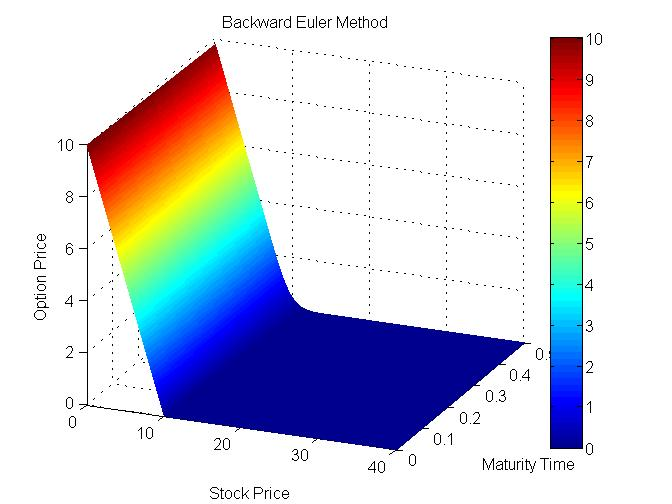
\includegraphics[height=3.5in,width=5in]{v_be.jpg}$\\

The surface of option price under Crank Nicolson Methods:\\
$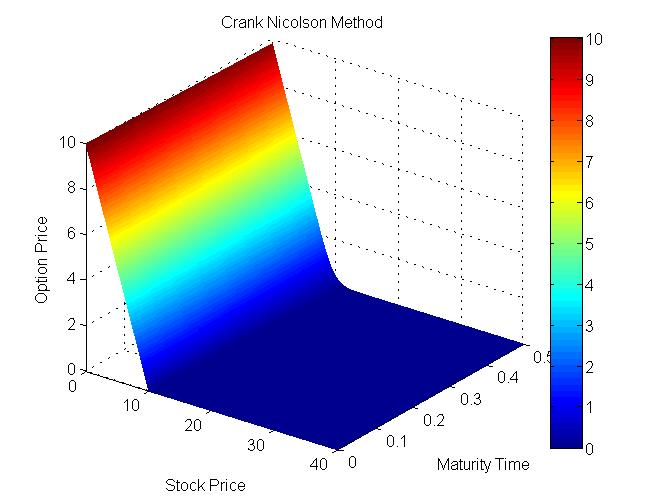
\includegraphics[height=3.5in,width=5in]{v_cn.jpg}$\\

The surface of option price under Ranacher Smooth Methods:\\
$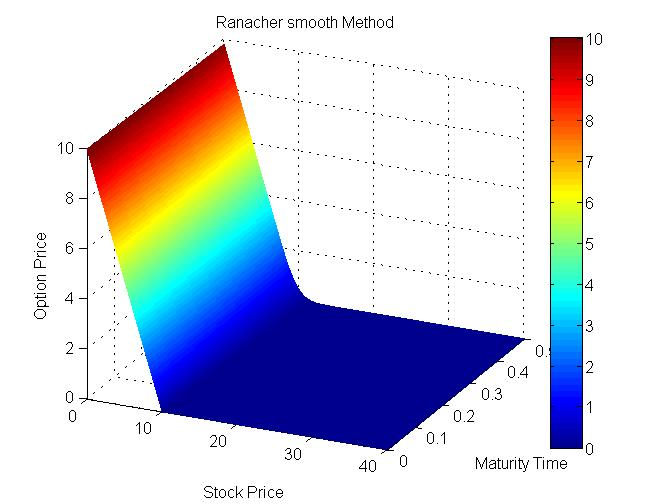
\includegraphics[height=3.5in,width=5in]{v_rs.jpg}$\\

The option price under different stock prices of Black Scholes method:\\
$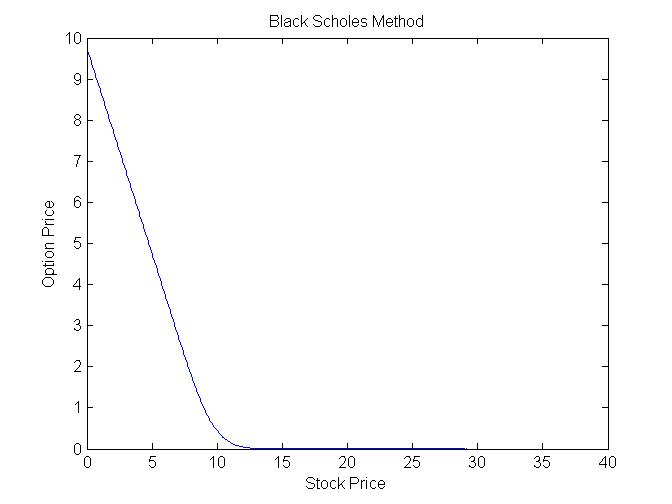
\includegraphics[height=3.5in,width=5in]{option_price_bs.jpg}$\\

The option price under different stock prices of Backward Euler method:\\
$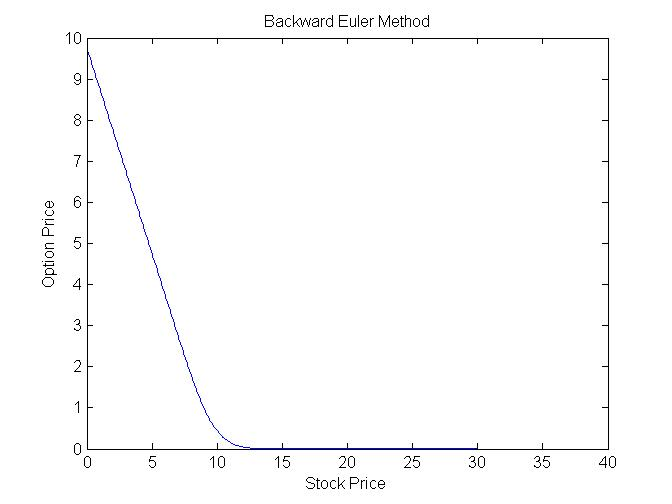
\includegraphics[height=3.5in,width=5in]{option_price_be.jpg}$\\

The option price under different stock prices of Crank Nicolson method:\\
$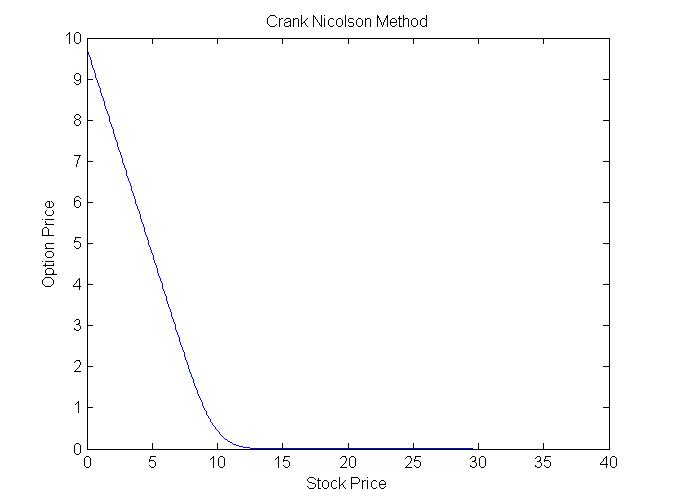
\includegraphics[height=3.5in,width=5in]{option_price_cn.jpg}$\\

The option price under different stock prices of Ranacher Smooth method:\\
$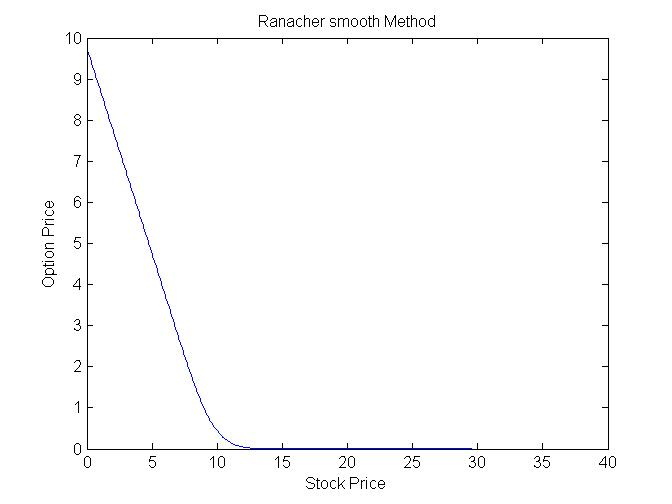
\includegraphics[height=3.5in,width=5in]{option_price_rs.jpg}$\\



\textbf{Delta:}\\
The Delta of option price under Black Scholes Methods:\\
$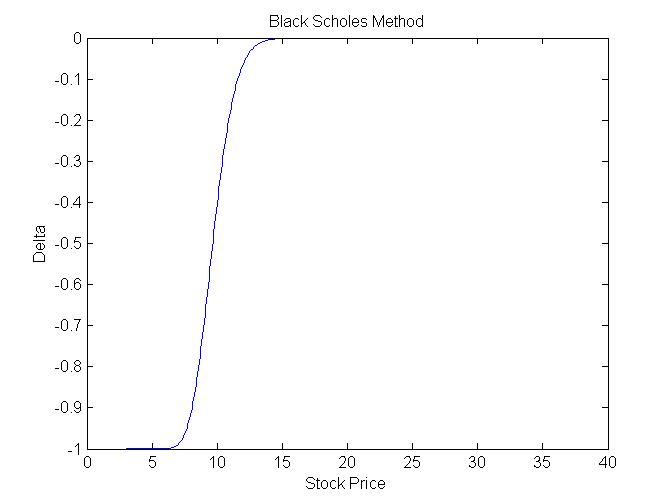
\includegraphics[height=3.5in,width=5in]{delta_bs.jpg}$\\

The Delta of option price under Backward Euler Methods:\\
$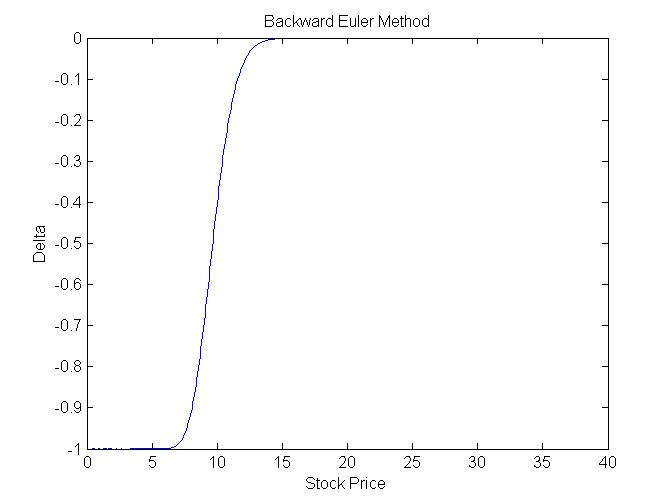
\includegraphics[height=3.5in,width=5in]{delta_be.jpg}$\\

The Delta of option price under Crank Nicolson Methods:\\
$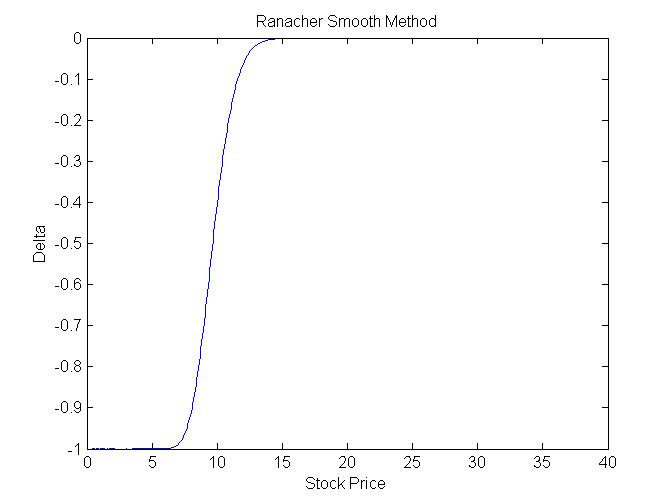
\includegraphics[height=3.5in,width=5in]{delta_cn.jpg}$\\

The Delta of option price under Ranacher Smooth Methods:\\
$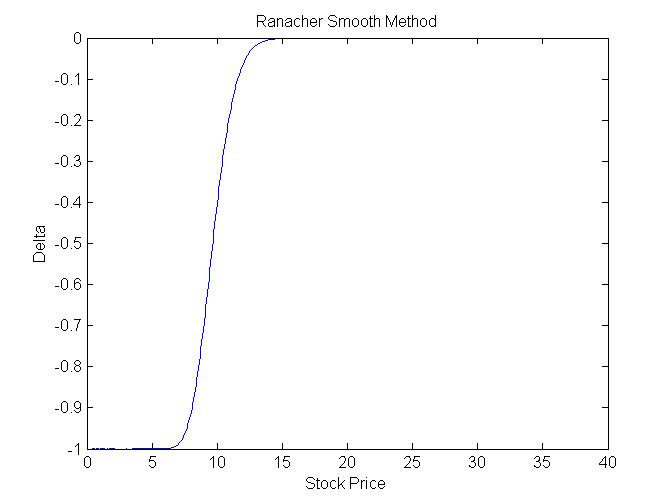
\includegraphics[height=3.5in,width=5in]{delta_rs.jpg}$\\

\textbf{Gamma:}\\
The Gamma of option price under Black Scholes Methods:\\
$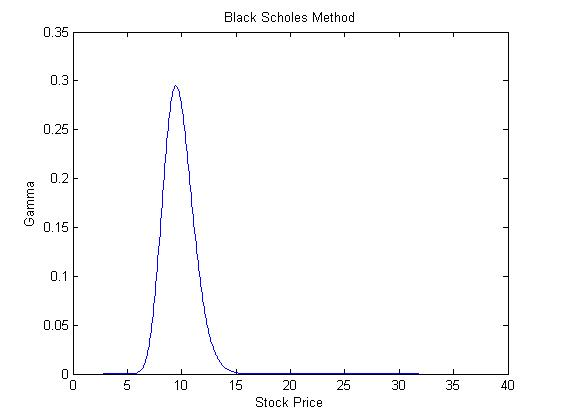
\includegraphics[height=3.5in,width=5in]{gamma_bs.jpg}$\\

The Gamma of option price under Backward Euler Methods:\\
$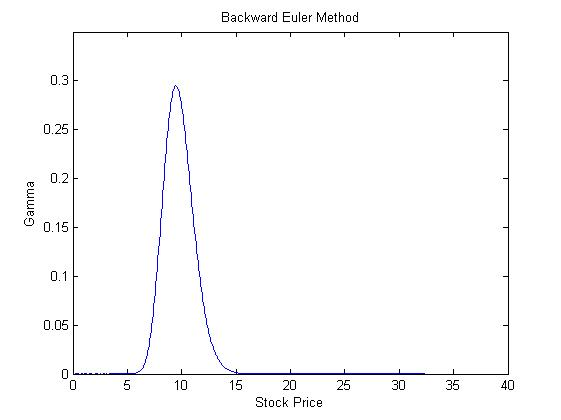
\includegraphics[height=3.5in,width=5in]{gamma_be.jpg}$\\

The Gamma of option price under Crank Nicolson Methods:\\
$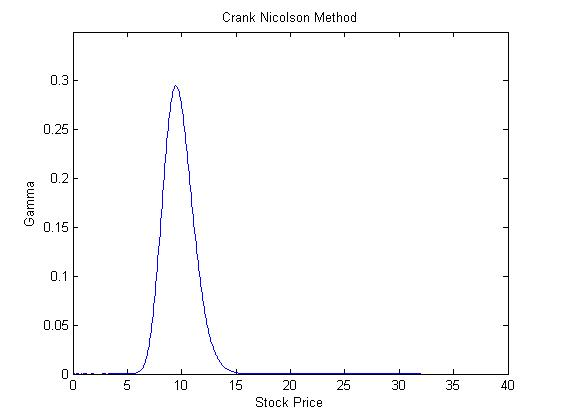
\includegraphics[height=3.5in,width=5in]{gamma_cn.jpg}$\\

The Gamma of option price under Ranacher Smooth Methods:\\
$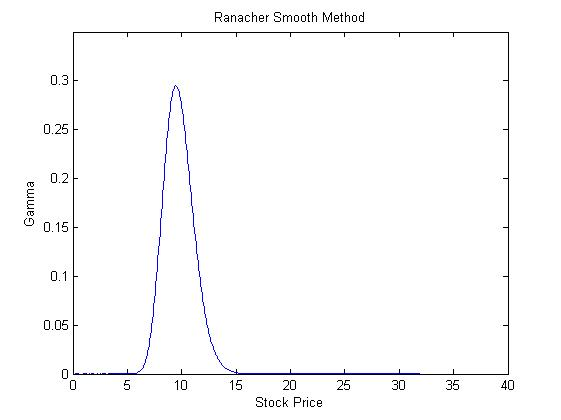
\includegraphics[height=3.5in,width=5in]{gamma_rs.jpg}$\\

\textbf{Vega:}
The Vega of option price under Black Scholes Methods:\\
$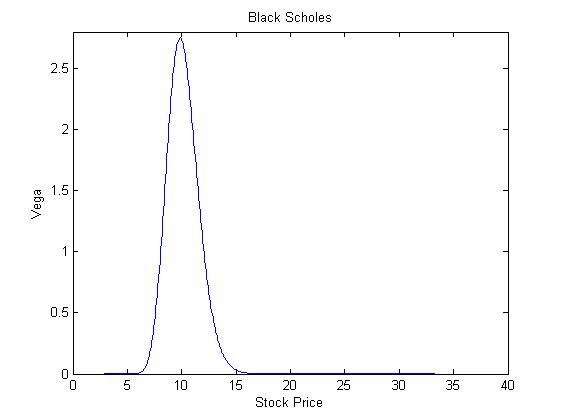
\includegraphics[height=3.5in,width=5in]{vega_bs.jpg}$\\

The Vega of option price under Backward Euler Methods:\\
$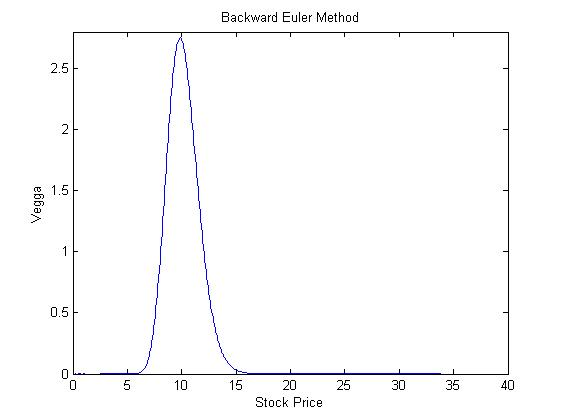
\includegraphics[height=3.5in,width=5in]{vega_be.jpg}$\\

The Vega of option price under Crank Nicolson Methods:\\
$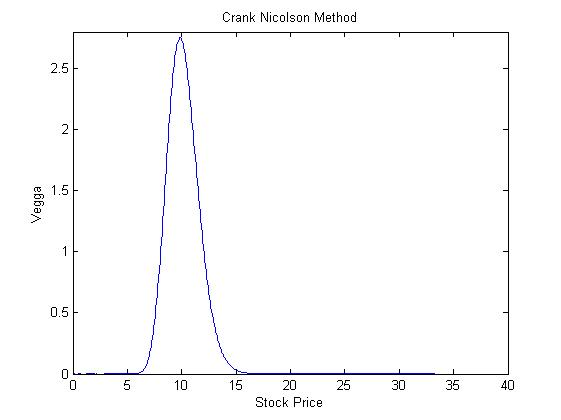
\includegraphics[height=3.5in,width=5in]{vega_cn.jpg}$\\

The Vega of option price under Ranacher Smooth Methods:\\
$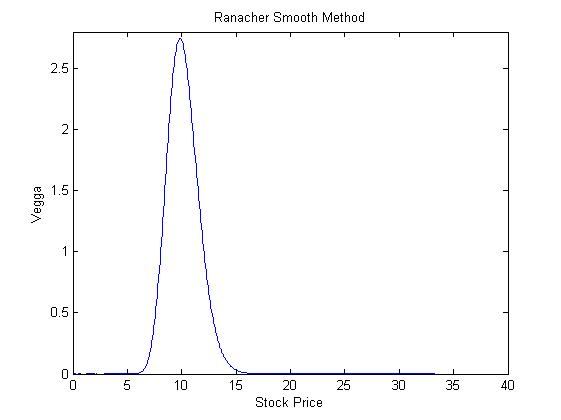
\includegraphics[height=3.5in,width=5in]{vega_rs.jpg}$\\


\textbf{Error Test}\\
First set the $N_x$ equal to 640 and see the error change based on the change of $N_t$\\

\begin{tabular}{|c|c|c|c|c|c|c|}
\hline
$N_t$&Backward&Rate& Crank Nicolson& Rate&Ranacher Smooth&Rate\\
\hline
20&	0.003594387&&	0.001567487&&		0.012230367& \\	
40&	0.001867687	&1.92& 	0.000132867&	11.80& 	0.006112979&	2.00\\
80	&0.00100197	&1.86 &	0.000135258	&0.98 	&0.003055939&	2.00\\
160	&0.000568873&	1.76& 	0.000137234&	0.99& 	0.001527832&	2.00\\
320	&0.000352555&	1.61 &	0.000137727	&1.00 &	0.000763881	&2.00\\
640	&0.000244465&	1.44 &	0.000137851	&1.00 	&0.000396422&	1.93\\
\hline
\end{tabular}

Next set the $N_t$ equal to 640 and see the error change based on the change of $N_x$\\

\begin{tabular}{|c|c|c|c|c|c|c|}
\hline
$N_x$&Backward&Rate& Crank Nicolson& Rate&Ranacher Smooth&Rate\\
\hline
20	&0.163436618	&&	0.163344756	&&	0.163662174	& \\
40	&0.040302554&	4.06& 	0.040159448&	4.07 &	0.040454358	&4.05\\
80	&0.009109848&	4.42 &	0.008996653&	4.46& 	0.009257477	&4.37\\
160	&0.00231537	&3.93 	&0.002206775&	4.08 	&0.00246187	&3.76\\
320	&0.00065681	&3.53 	&0.000552129&	4.00 	&0.000802989&	3.07\\
640	&0.000244465&	2.69 &	0.000137851&	4.01 &	0.000396422	&2.03\\
\hline
\end{tabular}

Finally change both $N_t$ and $N_s$\\
\begin{tabular}{|c|c|c|c|c|c|c|c|}
\hline
$N_x$&$N_t$&Backward&Rate& Crank Nicolson& Rate&Ranacher Smooth&Rate\\
\hline
20 &20&	0.166238921	&&	0.163327854&&	0.173703389&	\\
40&40	&0.042442619&	3.92 	&0.040143068&	4.07 &	0.044943594	&3.86\\
80	&80&0.009901673	&4.29 	&0.008993691	&4.46 	&0.011095262	&4.05\\
160	&160&0.002640911&	3.75 &	0.002206118	&4.08 	&0.003229567	&3.44\\
320	&320&0.000764333&	3.46 &	0.000552005	&4.00 	&0.001062514	&3.04\\
640	&640&0.000244465&	3.13 &	0.000137851	&4.00 	&0.000396422	&2.68\\
\hline
\end{tabular}

For the Greeks, We only test the convergence rate that both $N_x$ and $N_t$ are changed.

Delta:\\

\begin{tabular}{|c|c|c|c|c|c|c|c|}
\hline
$N_x$&$N_t$&Backward&Rate& Crank Nicolson& Rate&Ranacher Smooth&Rate\\
\hline
20&	20&	0.040638928&&		0.040343351	&&	0.042947343&	\\
40&	40&	0.012125597	&3.35& 	0.011656525&	3.46 &	0.012815246&	3.35\\
80&	80&	0.004392592	&2.76 &	0.004071524	&2.86 &	0.004890106	&2.62\\
160&	160&	0.001321169	&3.32& 	0.001036892	&3.93 &	0.003048254	&1.60\\
320&	320&	0.000460403	&2.87 &	0.000262897&	3.94 &	0.003048076&	1.00\\
640&	640&	0.000182361	&2.52 &	6.58197E-05&	3.99 &	0.003047988	&1.00\\
\hline
\end{tabular}

Gamma:\\

\begin{tabular}{|c|c|c|c|c|c|c|c|}
\hline
$N_x$&$N_t$&Backward&Rate& Crank Nicolson& Rate&Ranacher Smooth&Rate\\
\hline
20&	20&	0.07304392	&&	0.073453933	&&	0.071442482&	\\
40&	40&	0.035599504	&2.05& 	0.035458092	&2.07& 	0.0345424	&2.07\\
80&	80&	0.009692153	&3.67& 	0.009562398	&3.71 &	0.00911713	&3.79\\
160&	160&	0.002839872&	3.41& 	0.002495421&	3.83 &	0.006096616&	1.50\\
320&	320&	0.000856993&	3.31 &	0.000625908	&3.99& 	0.012192524	&0.50\\
640&	640&	0.00030478&	2.81& 	0.000156592&	4.00& 	0.02438434	&0.50\\
\hline
\end{tabular}

Vega:\\

\begin{tabular}{|c|c|c|c|c|c|c|c|}
\hline
$N_x$&$N_t$&Backward&Rate& Crank Nicolson& Rate&Ranacher Smooth&Rate\\
\hline
20&	20&	0.39866406	&&	0.440434356	&&	0.341570382	\\
40	&40&	0.264507211&	1.51 &	0.272835462&	1.61& 	0.245209753&	1.39\\
80	&80&	0.04499004&	5.88 &	0.049463898&	5.52 &	0.057953377	&4.23\\
160	&160&	0.01112004&	4.05 &	0.011662777&	4.24 &	0.020572162&	2.82\\
320	&320&	0.003324887&	3.34 &	0.002888742&	4.04& 	0.007843445&	2.62\\
640	&640&	0.001170097&	2.84 &	0.000721944	&4.00 &	0.00334992&	2.34\\

\hline
\end{tabular}



\end{homeworkProblem}

\begin{homeworkProblem}
Re do the problem 1 for the Binary option.
\textbf{Binary put option:}

The binary put option is that the payoff will be 1 if the maturity time stock price is lower than the strike price,otherwise it will be 0;\\
All the other assumptions are same with the vanilla put option.So we can rewrite the formula as follows:\\\\
Note that the boundary conditions changed.\\
$\left \{
\begin{tabular}{l}
$V_t+\frac{\sigma^2S^2}{2}V_{SS}+rSV_s - rV=0$\\
$V(0,t)=e^{-r(T-t)}$\\
$V(\infty,t)=0$\\
$V(S,T)=I_{\{S\leq K\}}$
\end{tabular}
\right.$

\textbf{Close form solution of the binary put:}
The Black-Scholes formula for binary put option is:\\

\begin{flalign*}
-e^{-r(T-t)}N(-d_2)
\end{flalign*}

where the $N(x)$ here is the cumulative function of standard normal distribution:\\

\textbf{Delta:}\\
\begin{flalign*}
-\frac{e^{-r(T-t)}N'(d_2)}{\sigma S\sqrt(T-t)}
\end{flalign*}

\textbf{Gamma:}\\
\begin{flalign*}
-\frac{e^{-r(T-t)}d_1N'(d_2)}{\sigma^2 S^2(T-t)}
\end{flalign*}

\textbf{Vega:}\\
\begin{flalign*}
-e^{-r(T-t)}N'(d_2)\frac{d_1}{\sigma}
\end{flalign*}

\textbf{Option price:}\\
We still used $E^*=\$10$, $r^*=0.05/yr$, $\sigma^*=0.20/yr$ T=0.5 as the example to build our model. \\
The number of time steps and the number of stock price steps are both equal to 640


The surface of option price under Backward Euler Methods:\\
$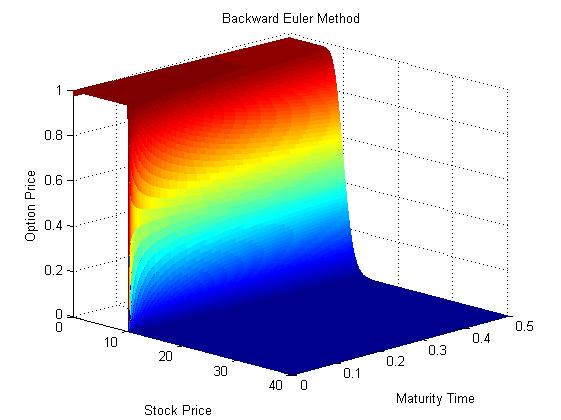
\includegraphics[height=3.5in,width=5in]{binary_v_be.jpg}$\\

The surface of option price under Crank Nicolson Methods:\\
$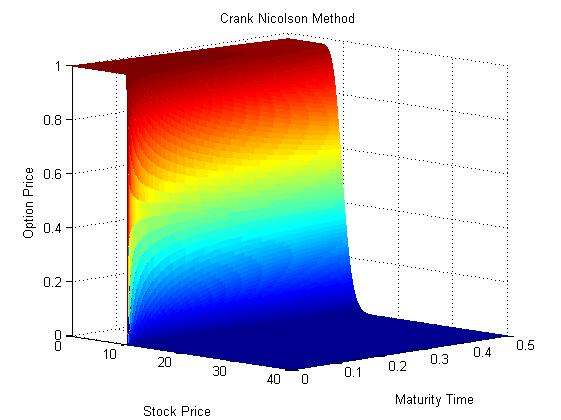
\includegraphics[height=3.5in,width=5in]{binary_v_cn.jpg}$\\

The surface of option price under Ranacher Smooth Methods:\\
$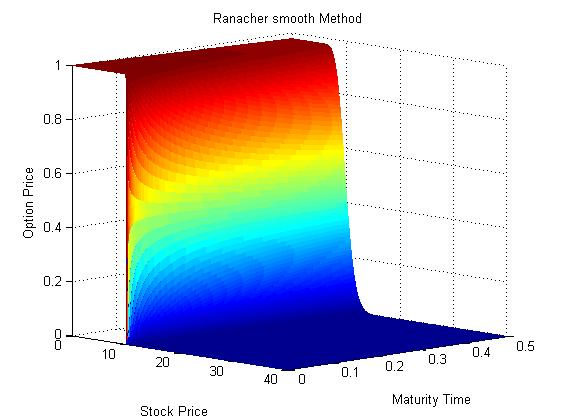
\includegraphics[height=3.5in,width=5in]{binary_v_rs.jpg}$\\


The option price under different stock prices of Black Scholes method:\\
$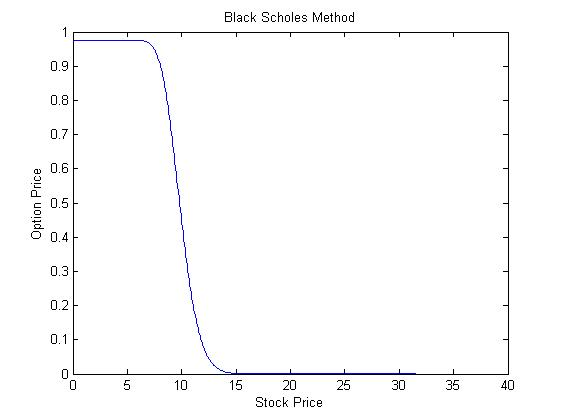
\includegraphics[height=3.5in,width=5in]{binary_option_price_bs.jpg}$\\

The option price under different stock prices of Backward Euler method:\\
$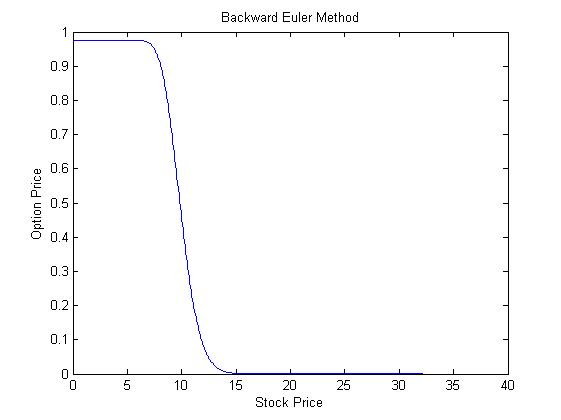
\includegraphics[height=3.5in,width=5in]{binary_option_price_be.jpg}$\\

The option price under different stock prices of Crank Nicolson method:\\
$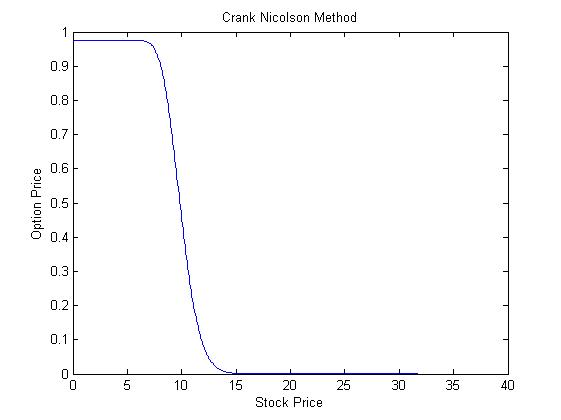
\includegraphics[height=3.5in,width=5in]{binary_option_price_cn.jpg}$\\

The option price under different stock prices of Ranacher Smooth method:\\
$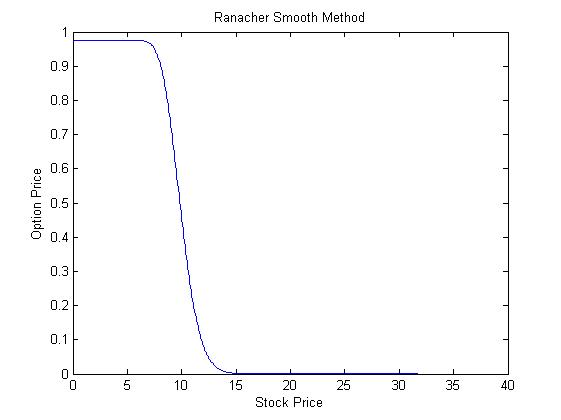
\includegraphics[height=3.5in,width=5in]{binary_option_price_rs.jpg}$\\

\textbf{Delta:}\\
The Delta of option price under Black Scholes Methods:\\
$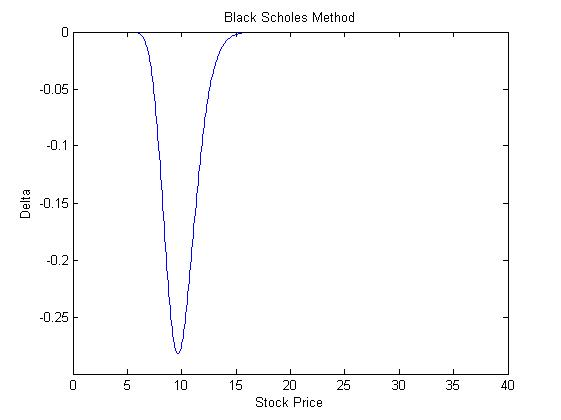
\includegraphics[height=3.5in,width=5in]{binary_delta_bs.jpg}$\\

The Delta of option price under Backward Euler Methods:\\
$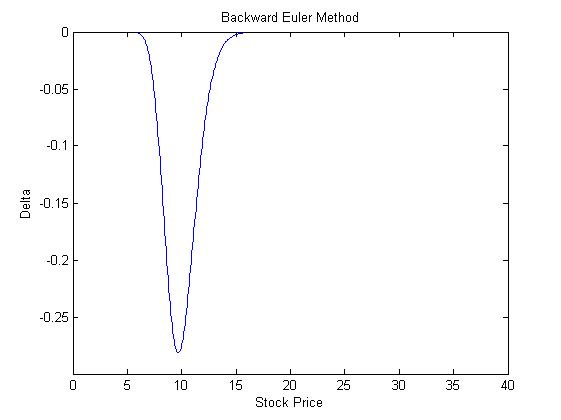
\includegraphics[height=3.5in,width=5in]{binary_delta_be.jpg}$\\

The Delta of option price under Crank Nicolson Methods:\\
$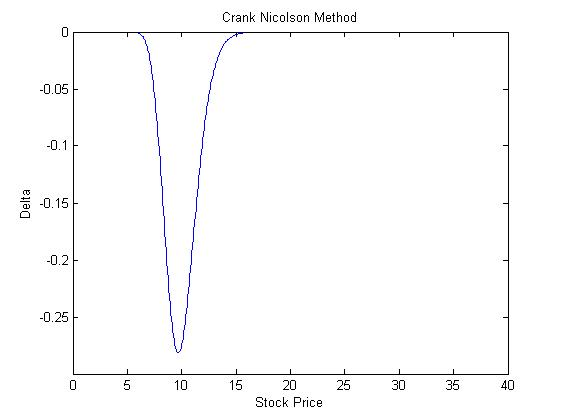
\includegraphics[height=3.5in,width=5in]{binary_delta_cn.jpg}$\\

The Delta of option price under Ranacher Smooth Methods:\\
$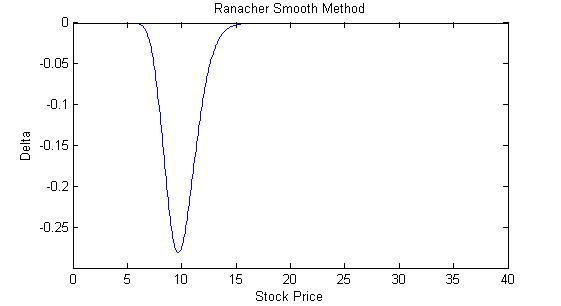
\includegraphics[height=3.5in,width=5in]{binary_delta_rs.jpg}$\\

\textbf{Gamma:}\\
The Gamma of option price under Black Scholes Methods:\\
$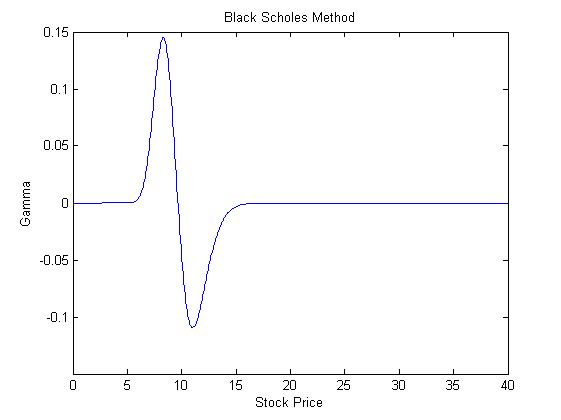
\includegraphics[height=3.5in,width=5in]{binary_gamma_bs.jpg}$\\

The Gamma of option price under Backward Euler Methods:\\
$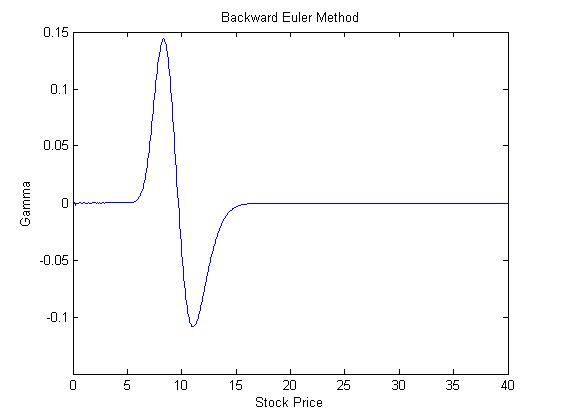
\includegraphics[height=3.5in,width=5in]{binary_gamma_be.jpg}$\\

The Gamma of option price under Crank Nicolson Methods:\\
$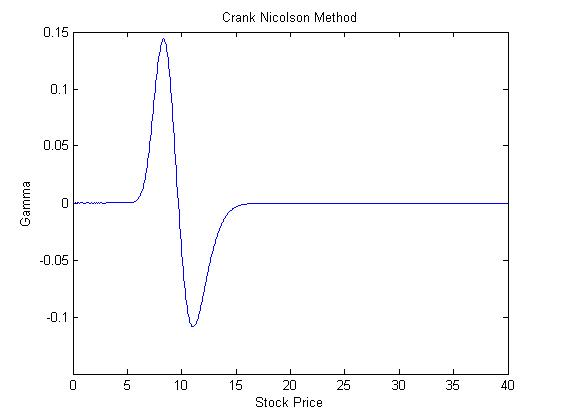
\includegraphics[height=3.5in,width=5in]{binary_gamma_cn.jpg}$\\

The Gamma of option price under Ranacher Smooth Methods:\\
$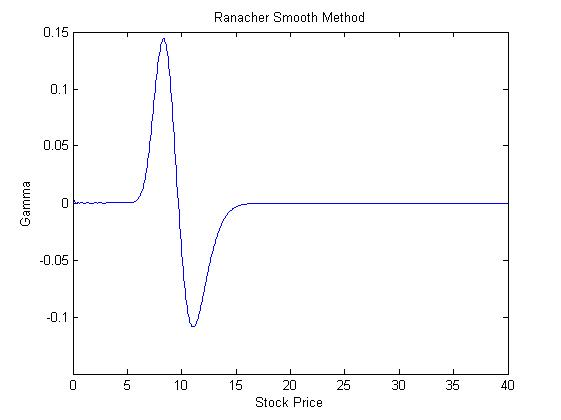
\includegraphics[height=3.5in,width=5in]{binary_gamma_rs.jpg}$\\

\textbf{Vega:}
The Vega of option price under Black Scholes Methods:\\
$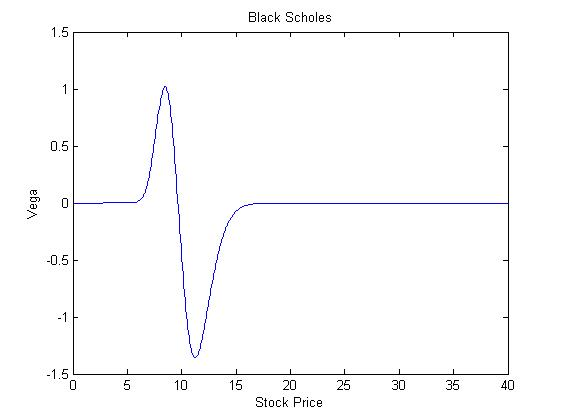
\includegraphics[height=3.5in,width=5in]{binary_vega_bs.jpg}$\\

The Vega of option price under Backward Euler Methods:\\
$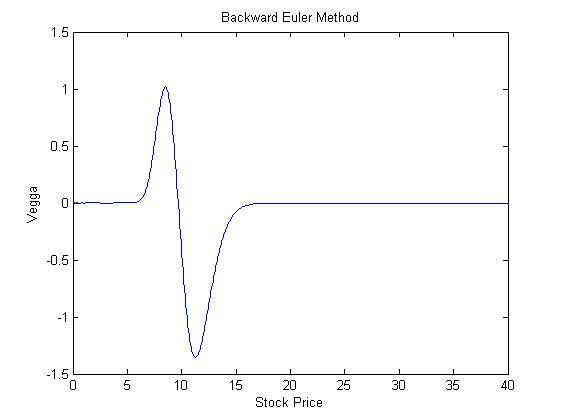
\includegraphics[height=3.5in,width=5in]{binary_vega_be.jpg}$\\

The Vega of option price under Crank Nicolson Methods:\\
$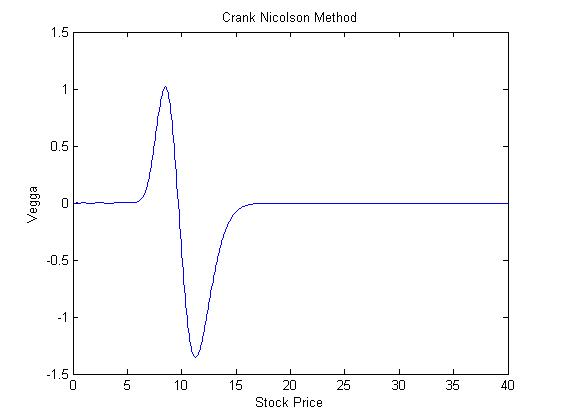
\includegraphics[height=3.5in,width=5in]{binary_vega_cn.jpg}$\\

The Vega of option price under Ranacher Smooth Methods:\\
$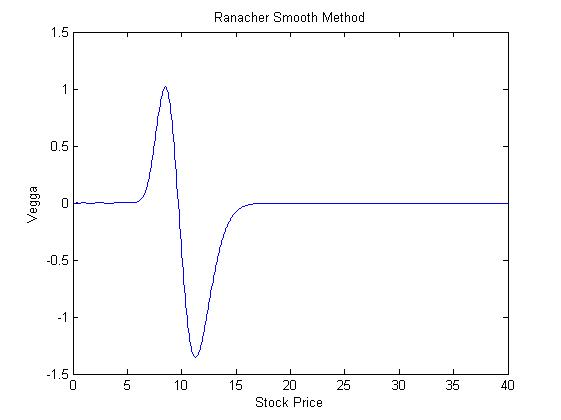
\includegraphics[height=3.5in,width=5in]{binary_vega_rs.jpg}$\\

\textbf{Error Test:}\\
We increased both the $N_x$ and $N_t$ from 20 to 640, to see the convergence rate of different methods for the binary put option.

1)For the put option price:\\

\begin{tabular}{|c|c|c|c|c|c|c|c|}
\hline
$N_x$&$N_t$&Backward&Rate& Crank Nicolson& Rate&Ranacher Smooth&Rate\\
\hline
20&	20&	0.317074957&&		0.314437672&&		0.322944148&	\\
40&	40&	0.150341433&	2.11& 	0.148175535&	2.12& 	0.151402278&	2.13\\
80&	80&	0.069756168&	2.16& 	0.0693145&	2.14& 	0.070194038&	2.16\\
160&	160&	0.034760674&	2.01& 	0.034475478&	2.01& 	0.035016767&	2.00\\
320&	320&	0.017298542&	2.01& 	0.017207956&	2.00& 	0.017418478&	2.01\\
640&	640&	0.008643274&	2.00& 	0.008598123&	2.00& 	0.00869713&	2.00\\
\hline
\end{tabular}

2) For the Delta:\\

\begin{tabular}{|c|c|c|c|c|c|c|c|}
\hline
$N_x$&$N_t$&Backward&Rate& Crank Nicolson& Rate&Ranacher Smooth&Rate\\
\hline
20	&20&	0.096672268&&		0.096032301&&		0.098693105&	\\
40&	40&	0.077343851	&1.25& 	0.076095613&	1.26 &	0.076609725&	1.29\\
80	&80&	0.038565233&	2.01 &	0.03756055&	2.03& 	0.038250679&	2.00\\
160	&160&	0.018763329&	2.06 &	0.018244999&	2.06& 	0.018504687&	2.07\\
320	&320&	0.009159206&	2.05 &	0.008909075&	2.05& 	0.009012556&	2.05\\
640	&640&	0.004519495&	2.03 &	0.004394301&	2.03& 	0.004449629&	2.03\\
\hline
\end{tabular}

3) For the vega:\\
\begin{tabular}{|c|c|c|c|c|c|c|c|}
\hline
$N_x$&$N_t$&Backward&Rate& Crank Nicolson& Rate&Ranacher Smooth&Rate\\
\hline
20&	20&	1.419941566&&		1.444646893&&		1.440652837&	\\
40&	40&	0.943121636&	1.51& 	0.931003917&	1.55 &	0.954989352&	1.51\\
80&	80&	0.364156019&	2.59& 	0.36099817&	2.58& 	0.366642911&	2.60\\
160&	160&	0.179932815&	2.02& 	0.178287731&	2.02 &	0.18146443&	2.02\\
320&	320&	0.088114546&	2.04& 	0.087399967&	2.04 &	0.088831093&	2.04\\
640&	640&	0.043696289&	2.02& 	0.043363191&	2.02 &	0.04404213&	2.02\\

\hline
\end{tabular}

We found that the value and greeks of binary put options are around first order convergence rate under all three methods.\\
\\
\begin{algorithm}
\DontPrintSemicolon
\Begin{
$x \longleftarrow x_0$\\
\For{k = 1 to maxiter}{
$rmax \longleftarrow 0$\\
\For {j = 1 to N-1}
{ $r= y_j- (l_j x_{j-1}+d_jx_j+u_jx_{j+1})$\\
  $x_{test}=x_j+\omega r /d_j$\\
  \If{$x_{test}>payoff_j$}{
      $x_j=x_{test}$\\
      $rmax=max(rmax,|r|)$}
  \Else
 {$x_j=payoff_j$}
 
 \If{$r_{max}<Tol$}
 {exit}
 }
}
}
\caption{PSOR Algoithm\label{IR}}
\end{algorithm}

\end{homeworkProblem}

\end{document} 